\documentclass[a4paper,10pt]{article}
\usepackage[utf8]{inputenc} 
\usepackage{rfi}
\usepackage{helvet}
\usepackage{xspace}
\usepackage{listings}
\usepackage{amsmath}
\usepackage{amssymb}
\usepackage{minted}
\usepackage{enumerate}
\usepackage[shortlabels]{enumitem}
\renewcommand{\familydefault}{\sfdefault}

\newcommand\AS[1]{\textcolor{green}{\emph{FK: #1}}}

\newcommand\key[1]{\textbf{#1}}
\newcommand\opt[1]{[{#1}]}
\newcommand\nt[1]{<{#1}>}

%%%%%%%%%%%%%%%%%%%%%%%%%%%%%%%%%%%%%%%%%%%%%%%%%%%%%%%%%%%%%%%%%%%%%%%%%%%%%%
\workpackageNumber{1}
\workpackageName{Software Specification}
\taskNumber{2.1}
\taskName{Define Agile Methodology}
\deliverableNumber{2}
\deliverableTitle{RadiantIQ Agile Methodology}
%Information: deliverableRunningTitle is used for the page footer, so try to write a short title!
\deliverableRunningTitle{RadiantIQ Agile Methodology}
\deliverableResponsible{RadiantIQ develop team}
\deliverableVersion{2.0}
\deliverableStatus{Completed}
\deliverableAuthors{Lorenzo Cattai, Gabriele Pernici, Anh Tu Duong, Lorenzo Negut}
\dueDate{27/05/2024}
\submissionDate{27/05/2024}
\deliverableType{DOCUMENT}
%%%%%%%%%%%%%%%%%%%%%%%%%%%%%%%%%%%%%%%%%%%%%%%%%%%%%%%%%%%%%%%%%%%%%%%%%%%%%%


\setcounter{secnumdepth}{5}
\setcounter{tocdepth}{5}

% \usepackage{xspace}

\newcommand{\sysml}{\emph{SysML}\xspace}
\newcommand{\uml}  {\emph{UML}\xspace}


\begin{document}
	\thispagestyle{empty}

\begin{center}

\begin{figure}
\centering
  \begin{subfigure}[b]{0.4\textwidth}
    
\includegraphics[width=0.7\linewidth]{images/radiantiq}
  \end{subfigure}
 \hfill
  \begin{subfigure}[b]{0.4\textwidth}
    
\includegraphics[width=0.8\linewidth]{images/unitn}
  \end{subfigure}
\end{figure}

\vspace{1.5cm}

\arrayrulecolor{RFIGreen}


{\setlength{\extrarowheight}{2pt}
\begin{tabular}{|rp{10cm}|}
\hline
\textcolor{RFIGreen}{\small\bf\em ~~~Project's acronym:} & {\small RADIANTIQ}\\

\textcolor{RFIGreen}{\small\bf\em Project's title:} & {\small RadiantIQ}\\

\textcolor{RFIGreen}{\small\bf\em Start date:} & {\small 08/03/2024}\\
\textcolor{RFIGreen}{\small\bf\em Finish date:} & {\small DD/MM/YYYY}\\
\hline
\end{tabular}
}
\vspace{2cm}

{\huge\bf D\theDeliverableNumber\ - \theDeliverableTitle}

\vspace{2cm}

{\setlength{\extrarowheight}{2pt}
\begin{tabular}{rp{10cm}}
\textcolor{RFIGreen}{\bf WP\theWorkpackageNumber:} & \theWorkpackageName\\
\textcolor{RFIGreen}{\bf Task \theTaskNumber:} & \theTaskName\\
\textcolor{RFIGreen}{\bf Submission date:} & \theDueDate\\
\textcolor{RFIGreen}{\bf Responsible:} & \theDeliverableResponsible\\
\textcolor{RFIGreen}{\bf Version:} & \theDeliverableVersion\\
\textcolor{RFIGreen}{\bf Status:} & \theDeliverableStatus\\
\textcolor{RFIGreen}{\bf Author(s):} & \theDeliverableAuthors\\
%\textcolor{BurntOrange}{\bf Reviewer(s):} & \theDeliverableReviewers\\
\textcolor{RFIGreen}{\bf Deliverable type:} & \theDeliverableType\\
\end{tabular}
}

\end{center}

\newpage

	% % !TEX root = ../d3.5.tex
\textcolor{RFIGreen}{\Large\bf Version list:}

\arrayrulecolor{black}

\begin{center}

{\setlength{\extrarowheight}{6pt}
\rowcolors[\hline]{1}{white}{gray}
\begin{tabular}{|p{1.5cm}|p{4.5cm}|p{2.5cm}|p{5.5cm}|}
\hline
{\small\bf Version} & {\small\bf Authors} & {\small\bf Date} & {\small\bf Description}\\
\hline
0.1 & Anh Tu Duong & 03/05/2024  & Define the scheme of the document \\
\end{tabular}
}

\end{center}

\newpage
%%% Local Variables:
%%% mode: latex
%%% TeX-master: "main"
%%% End:

	
	\tableofcontents
	\newpage
	
	% \textcolor{RFIGreen}{\Large\bf Acronyms}

\begin{center}

\begin{tabular}{|p{5cm}|p{9cm}|}
\hline
{\small\bf Acronym} & {\small\bf Description}\\
\hline

FRS & Functional Requirement Specification\\
FSD & Functional Specification Document\\
FLOSS & Free/Libre Open Source Software\\
LLMs & Large Language Models\\
UML & Unified Modeling Language\\
UniTn & University of Trento\\

\hline

\end{tabular}

\end{center}

\newpage

	
	\newpage
	\section{Introduction} \label{introduction}
The project consists in a platform providing a better learning experience for scientific subjects. The idea is to include standard formal explanations of topics (with associated exercises) accompanied by a small number of interactive minigames. To better involve the students, each exercise will be put in an AI generated context (e.i. a phisics problem related to speeds and distances could be told using the story of Achilles and the turtoise). Moreover, the formal explanations can be genrated by an AI, uploaded by a professor or by a combination of the two. Lastly, AI is used to suggest which topics should be revised for the students using the platform.

	\newpage
	\section{Architecture description} \label{architecture_description}


	\newpage
	\section{API Definition} \label{api_definition}


	\newpage
	\section{Product backlog} \label{product_backlog}


	\newpage
	\section{Definition of tests} \label{definition_of_tests}

	\subsection{Overview}

		\subsubsection{Importance of Testing}

		Testing plays a critical role in ensuring the functionality, usability, and security of RadiantIQ. As an platform, it must not only meet industry standards for software quality but also provide a reliable and efficient learning experience for our users. Comprehensive testing helps identify and address issues early in the development process, reducing critical issues impacting the user experience post-deployment.

		\subsubsection{Scope}

		This document outlines the testing strategy for RadianIQ, detailing the objectives, testing types, approach, test cases, test environment, test execution process, risks, and mitigation strategies. It serves as a guideline for the testing team, developers, and stakeholders involved in the development and quality assurance of the application. RadiantIQ test development will be based on the outlined below and encourage to use mixed testing methods to ensure the quality of the platform.
		
		
	\subsection{Testing Objectives}
	
		\subsubsection{Goals of the Testing Strategy}
		
		The primary objective is to ensure that the platform meets the highest standards of quality, reliability, and security. Specifically, it aims to:
		
		\begin{itemize}
			\item Verify the functionality of all features: Ensure that each function of the web application, including course and class management, user registration, content delivery, and communication features, works as intended without any errors or unexpected behavior.
			\item Usability and accessibility: Evaluate the user-friendliness and accessibility of the platform to ensure that users can navigate the application easily and perform their tasks efficiently.
			\item Ensure compatibility across different environments: Confirm that RadianIQ is compatible with various browsers (e.g., Chrome, Firefox, Safari), devices (e.g., desktops, laptops, tablets, smartphones), and operating systems (e.g., Windows, macOS, iOS, Android).
			\item Evaluate performance: Test the responsiveness and scalability of the application to ensure that it can handle multiple users accessing the platform simultaneously and perform well under high peak.
			\item Identify and mitigate security vulnerabilities: Conduct thorough security testing to identify potential vulnerabilities, such as data breaches, unauthorized access, and injection attacks, and implement measures to mitigate these risks and protect user data.
			\item Ensure integration between components: Validate the interaction between different components and modules of the platform to ensure seamless functionality and data exchange.
		\end{itemize}

		
	\subsection{Testing Types}
		
		\subsubsection{Functional Testing (Black-box Testing)}
		
		Functional testing ensures that each function of RadianIQ works as expected. This involves testing individual features and functionalities to verify that they meet the specified requirements, including:
		
		\begin{itemize}
			\item Course Management: Testing the creation, editing, and deletion of courses, including features such as adding course materials, setting up assessments, and managing enrollments.
			\item Class Management: Testing the creation, editing, and deletion of classes, including features such as creating class sessions, managing student registrations, tracking student progress, and grading assignments.
			\item User Registration and Authentication: Testing the registration process for all the user roles, as well as the login and authentication mechanisms to ensure secure access to the platform.
			\item Content Delivery: Testing the delivery of course content, including multimedia materials, documents, mini games, and lectures, to ensure they are accessible and functional.
			\item Communication Features: Testing messaging systems, discussion forums, and collaboration tools to ensure smooth communication and interaction between users.
		\end{itemize}

		\subsubsection{Structural Testing (White-box Testing)}

		Structural testing, or white-box testing, involves examining the internal structure and code of the e-learning web application to validate its logic, algorithms, and internal pathways. This testing type ensures the reliability, security, and maintainability of the application's underlying codebase. Key aspects to test include:

		\begin{itemize}
			\item Code Coverage: Verify that all code paths, including branches, loops, and conditionals, are executed and tested to achieve high code coverage.
			\item Data Validation: Validate input data to prevent security vulnerabilities such as SQL injection, cross-site scripting (XSS), and data manipulation attacks.
			\item Error Handling: Ensure robust error handling mechanisms are in place to gracefully handle exceptions, invalid inputs, and unexpected scenarios without crashing the application.
			\item Performance Optimization: Analyze code performance to identify and optimize inefficient algorithms, database queries, and resource-intensive operations for improved scalability and responsiveness.
		\end{itemize}
		
		\subsubsection{Usability Testing}
		
		Usability testing focuses on assessing the user-friendliness and accessibility of the platform. This involves evaluating the interface design, navigation flow, and overall user experience to ensure that users can easily accomplish their tasks and achieve their learning objectives. Usability testing includes:
		
		\begin{itemize}
			\item Navigation Testing: Evaluating the navigation flow within the application to ensure that users can easily find and access the desired features and content.
			\item Accessibility Testing: Ensuring that the platform is accessible to users with disabilities, including compliance with accessibility standards such as WCAG (Web Content Accessibility Guidelines).
			\item User Feedback Analysis: Gathering feedback from users through surveys, interviews, or usability testing sessions to identify areas for improvement in the user interface and experience.
		\end{itemize}
		
		\subsubsection{Compatibility Testing}
		
		Compatibility testing ensures that RadianIQ is compatible across different browsers, devices, and operating systems. This involves testing the application on various combinations of browsers (e.g., Chrome, Firefox, Safari), devices (e.g., desktops, laptops, tablets, smartphones), and operating systems (e.g., Windows, macOS, iOS, Android) to ensure consistent performance and functionality.
		
		\subsubsection{Performance Testing}
		
		Performance testing evaluates the responsiveness and scalability of the platform under various loads. This involves testing the application's performance metrics such as response time, throughput, and resource utilization to ensure optimal performance under normal and peak usage conditions. Performance testing includes:
		
		\begin{itemize}
			\item Load Testing: Simulating multiple users accessing the platform simultaneously to assess its response time and behavior under heavy loads.
			\item Stress Testing: Pushing the system beyond its normal capacity to identify its breaking point and evaluate its ability to recover under stress.
			\item Scalability Testing: Testing the application's ability to scale resources dynamically to accommodate increasing user loads without degradation in performance.
		\end{itemize}
		
		\subsubsection{Security Testing}
		
		Security testing aims to identify and mitigate potential security vulnerabilities in the platform. This involves testing the application for vulnerabilities such as data breaches, unauthorized access, injection attacks, and XSS (cross-site scripting) attacks. Security testing includes:
		
		\begin{itemize}
			\item Vulnerability Assessment: Identifying potential security vulnerabilities through automated scanning tools and manual code reviews.
			\item Penetration Testing: Simulating real-world attacks to exploit vulnerabilities and assess the effectiveness of security controls and countermeasures.
			\item Data Protection Testing: Ensuring that sensitive user data such as personal information, grades, and assessment results are securely stored, transmitted, and accessed according to privacy regulations and best practices.
		\end{itemize}

		
	\subsection{Testing Method Approach}

		\subsubsection{V-Model Testing}

		\begin{figure}[H]
			\centering
			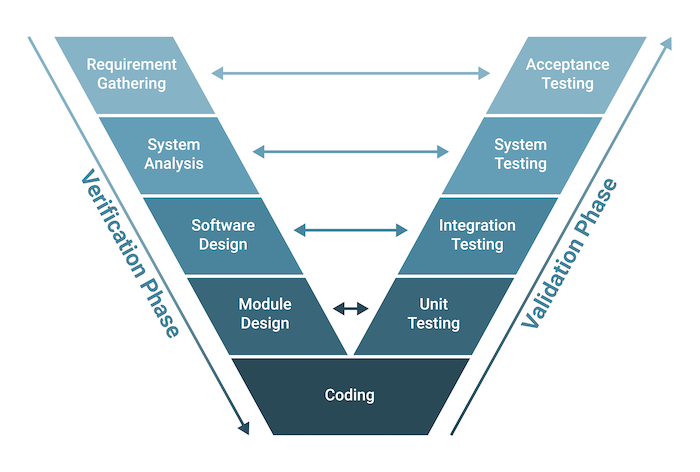
\includegraphics[width=0.55\linewidth]{images/v-model-testing.png}
			\caption{V-model testing}
			\label{fig:v-model-testing}
		\end{figure}

		The V-Model testing approach aligns testing activities with corresponding development phases, emphasizing the relationship between requirements, design, implementation, and testing. In the V-Model, each phase of the development lifecycle has a corresponding testing phase, ensuring comprehensive validation at each stage. The V-Model testing process includes:

		\begin{itemize}
			\item Acceptance Testing (Requirements Gathering): During the requirements gathering phase, acceptance testing focuses on validating the gathered requirements to ensure they are clear, complete, and consistent. This involves collaborating with stakeholders to define acceptance criteria and validate that the requirements accurately capture the needs of end-users and align with business objectives.
			\item System Testing (System Analysis): In the system analysis phase, system testing verifies the complete integrated system against the specified requirements and design specifications. This includes testing the system as a whole to ensure that all components function correctly together and meet the intended functionality, performance, and usability criteria.
			\item Integration Testing (Software Design): Integration testing validates the interaction and integration between individual software modules or components. It ensures that modules interact correctly, exchange data seamlessly, and function as expected within the larger system architecture. Integration testing verifies that the software design, including interfaces and dependencies, is implemented correctly and that modules work together harmoniously.
			modules.
			\item Unit Testing (Module Design): Unit testing focuses on validating the functionality of individual software modules or components in isolation. It verifies that each module performs its intended function according to the specified design and requirements. Unit tests are designed to test specific inputs, outputs, and internal logic of modules, ensuring that each unit operates correctly and meets its design specifications.
		\end{itemize}

		\subsubsection{Manual Testing}
		
		Manual testing involves human testers executing test cases and evaluating the application's behavior based on predefined criteria. This approach allows testers to identify visual inconsistencies, usability issues, and other aspects that may be challenging to automate. The manual testing process includes:
		
		\begin{itemize}
			\item Test Case Creation: Developing detailed test cases based on functional requirements and user stories.
			\item Test Execution: Performing manual tests according to the test cases, documenting observations, and verifying expected outcomes.
			\item Exploratory Testing: Conducting ad-hoc testing to explore the application and uncover potential issues that may not be covered by predefined test cases.
			\item Usability Testing: Engaging real users to evaluate the application's usability, accessibility, and overall user experience.
			\item Regression Testing: Repeating tests to ensure that new features or changes do not adversely affect existing functionalities.
		\end{itemize}
		
		\subsubsection{Automated Testing}
		
		Automated testing involves using software tools and frameworks to automate the execution of test cases, thereby increasing efficiency, repeatability, and coverage. This approach is particularly useful for repetitive tasks and regression testing. The automated testing process includes:
		
		\begin{itemize}
			\item Test Script Development: Writing test scripts using automated testing tools such as Selenium, Cypress, or TestComplete to simulate user interactions and verify expected behaviors.
			\item Test Suite Creation: Organizing test scripts into test suites based on functional areas or features for efficient execution and maintenance.
			\item Continuous Integration (CI) Integration: Integrating automated tests into the CI/CD pipeline to automatically trigger tests upon code changes and provide rapid feedback to developers.
			\item Cross-Browser and Cross-Platform Testing: Executing tests across different browsers, devices, and operating systems to ensure compatibility and consistent behavior.
			\item Performance Testing Automation: Utilizing tools like JMeter or Gatling for automating performance tests to simulate various load scenarios and analyze system performance metrics.
		\end{itemize}
		
		\subsubsection{Regression Testing}
		
		Regression testing ensures that new changes or enhancements do not introduce unintended side effects or break existing functionalities. The regression testing process includes:
		
		\begin{itemize}
			\item Test Case Maintenance: Updating existing test cases and creating new ones to accommodate changes in the application.
			\item Test Suite Prioritization: Prioritizing test cases based on their criticality and impact on the application to optimize testing efforts.
			\item Automated Regression Testing: Automating repetitive regression tests to ensure consistent and efficient validation of core functionalities.
			\item Manual Regression Testing: Performing manual regression tests for areas that are difficult to automate or require human judgment.
			\item Version Control Integration: Integrating regression tests with version control systems to track changes and ensure test coverage across different software versions.
		\end{itemize}
		
	
	\subsection{Test Environment}
	
		\subsubsection{Hardware Specifications}
		
		The test environment setup for RadianIQ should include hardware specifications that closely resemble the production environment to ensure accurate testing results. The hardware specifications may include:
		
		\begin{itemize}
			\item Server Configuration: Specifications for Render.com, server hosting the web application, including CPU, RAM, and storage capacity.
			\item Client Devices: Specifications for client devices used to access the application, such as desktop computers, laptops, tablets, and smartphones.
			\item Networking Equipment: Details of networking hardware such as routers, switches, and firewalls that may impact network performance and connectivity.
		\end{itemize}
		
		\subsubsection{Software Dependencies}
		
		The test environment should replicate the software dependencies of the production environment to ensure compatibility and accurate testing. This includes:
		
		\begin{itemize}
			\item Operating Systems: Versions of operating systems supported by the platform.
			\item Web Browsers: Versions of web browsers supported by the application, including Chrome, Firefox, Safari, and Edge.
			\item Database Systems: Versions of database management systems (DBMS) used by the application. In this case, MongoDB.
			\item Server Software: Versions of web servers, application servers, and other server software required to run the application.
		\end{itemize}
		
		\subsubsection{Network Configurations}
		
		Network configurations play an important role in testing the performance and reliability. The test environment should simulate real-world network conditions to evaluate the application's behavior under different scenarios. This includes:
		
		\begin{itemize}
			\item Internet Connectivity: Ensure stable internet connectivity with sufficient bandwidth to support concurrent user interactions.
			\item Firewall and Security Settings: Configure network security settings to simulate firewall rules and security protocols that may impact application access and communication.
			\item Load Balancing: Implement load balancing configurations to distribute traffic across multiple servers and assess scalability and performance under heavy loads.
			\item Latency and Packet Loss: Introduce latency and packet loss to simulate network congestion and assess application responsiveness and resilience.
		\end{itemize}
		
		\subsubsection{Data Sets for Testing}
		
		Data sets used for testing should represent realistic scenarios and volumes to validate the performance, scalability, and reliability of the platform. This includes:
		
		\begin{itemize}
			\item Sample Courses and Content: Populate the test environment with a variety of sample courses, lectures, mini games, and multimedia content to simulate real usage scenarios.
			\item User Data: Create test user accounts with different roles and varying levels of access permissions to test user registration, authentication, and authorization functionalities.
			\item Test Data Generation: Use data generation tools or scripts to create large volumes of test data to simulate realistic user interactions, such as enrollment in courses, participation in discussions, and submission of assignments.
		\end{itemize}
		
	\subsection{Bug Reporting and Tracking}
	
	Bug reporting and tracking are essential aspects of the test execution process, enabling testers to document and manage issues effectively. The bug reporting and tracking process includes:
	
	\begin{itemize}
		\item Defect Identification: Identify and document defects discovered during test execution, including detailed descriptions, steps to reproduce, and screenshots or logs.
		\item Defect Prioritization: Prioritize defects based on severity, impact on functionality, and business priority to focus on resolving critical issues first.
		\item Defect Management: Assign, track, and manage defects using a centralized defect tracking system or bug management tool to ensure transparency, accountability, and traceability throughout the defect lifecycle.
		\item Defect Resolution: Collaborate with development teams to investigate, triage, and resolve reported defects promptly, following established workflows and communication channels.
	\end{itemize}


\subsection{Test cases template}

Providing here the base test cases table, where each iteration will define more test cases.


\begin{longtable}{|c|m{1.5cm}|m{2.5cm}|m{2.5cm}|m{1.5cm}|m{2.5cm}|m{1.5cm}|m{1.5cm}|}
	\hline
	N. & Description & Test case data & Precondition & Dep. & Expected result & Actual result & Notes \\ \hline
	\endhead
	%
	0 & Login with unregisted user & Go to login page; insert username and password &  &  & A message is displayed "Invalid username or password". The login page is reload. &  &  \\ \hline
	1.1 & Register new user successfully & Go to login page; and insert firstname, lastname, email, username and password &  &  & A message is displayed "User created successfully". The dashboard is loaded. &  &  \\ \hline
	1.2 & Register new user failed & Go to login page; and insert firstname, lastname, email, username and password & - email or username is already used by another user. &  & A message is displayed "Email or username is not available". &  &  \\ \hline
	2.1 & Login with registed user successfully & Go to login page; insert username and password & user has already registerd &  & A message is displayed "Login successfully. Welcome back \{username\}". The dashboard is loaded. &  &  \\ \hline
	2.2 & Wrong password & Go to login page; insert username and wrong password &  &  & A message is displayed "Wrong password, please try again". &  &  \\ \hline
	2.3 & Login with empty or wrong username & Go to login page; insert wrong username &  &  & A message is displayed "Invalid username, please try again". &  &  \\ \hline
	3.1 & Logout successfully & Click Logout button & user has already logged in &  & A message is displayed "Logout successfully". The login page is reload. &  &  \\ \hline
	4.1 & Credential recovery & Go to "Recover" insert email &  &  & A message is displayed "An email with recovery info has been sent to your email". Send an email with credential info to the user email. The login page is reload. &  &  \\ \hline
	5.1 & Delete account & In Account Management, click "Delete Account"; insert password; click "Yes, I'm sure to delete my account" & user has already logged in &  & A form for user to choose the reasons why the user want to delete account displayed. The account deleted. The login page is reload. &  &  \\ \hline
	6.1 & Modify account successfully & In Account Management, click "Modify Account"; insert password; modify the allowed field & user has already logged in &  & A message is displayed "Modified successfully". The dashboard is reload. &  &  \\ \hline
	6.2 & Modify account failed & In Account Management, click "Modify Account"; insert password; leave any field empty & user has already logged in &  & A message is displayed "Modified not successfully". The dashboard is reload. &  &  \\ \hline
	7.1 & Modify secondary settings successfully & In Setting, modify secondary settings (e.g. theme, layout,...) & user has already logged in &  & A message is displayed "Modified successfully". The dashboard is reload. &  &  \\ \hline
	8.1 & Modify AI theming successfully & In AI theming option, inputs a prompt, confirm the modification & user has already logged in &  & A message is displayed "Modified AI theming successfully". The dashboard is reload. &  &  \\ \hline
	9.1 & Access profile and statistics & Selects the account display option & user has already logged in &  & The profile with all its statistics is displayed &  &  \\ \hline
	10.1 & Change user role & In "User Role" panel, select one of the allowed user roles & user has already logged in &  & The user role changed following by his dashboard role. &  &  \\ \hline
	11.1 & Create course & In "Course" panel, select "Create new course", fill the mandatory sections, click "Create new course" final button & user has already logged in, has the right to modify course &  & Course editor displayed "New course has been created" &  &  \\ \hline
	11.2 & Modify course & In "Course" panel, select "Modify course", fill the mandatory sections, click "Modify course" final button & user has already logged in, has the right to modify course &  & Course editor displayed "Course \{name\} has been modified" &  &  \\ \hline
	11.3 & Delete course & In "Course" panel, select "Modify course", click "delete course" & user has already logged in, has the right to modify course &  & Course editor displayed "Course \{name\} has been deleted" &  &  \\ \hline
	11.4 & Archive course & In "Course" panel, select "Modify course", click "Archive course" & user has already logged in, has the right to modify course &  & Course editor displayed "Course \{name\} has been archived" &  &  \\ \hline
	11.5 & View course & Select course from the dashboard & user has already logged in, has the right to access course &  & The course is displayed, along with the global rank-\\ ing if any minigame is present &  &  \\ \hline
	11.6 & Review course & Select course from the dashboard, leave a review (comment) for the\\ course & user has already logged in, has the right to access course &  & The review is added to the course &  &  \\ \hline
	12.1 & Create class & In "Class" panel, select "Create new Class", fill the mandatory sections, click "Create new Class" final button & user has already logged in, has the right to modify Class &  & Class editor displayed "New Class has been created" &  &  \\ \hline
	12.2 & Modify class & In "Class" panel, select "Modify Class", fill the mandatory sections, click "Modify Class" final button & user has already logged in, has the right to modify Class &  & Class editor displayed "Class \{name\} has been modified" &  &  \\ \hline
	12.2 & Terminate class & In "Class" panel, select "Modify Class", click "Terminate Class" final button & user has already logged in, has the right to modify Class &  & Class editor displayed "Class \{name\} has been terminated" &  &  \\ \hline
	12.3 & Archive class & In "Class" panel, select "Modify Class", click "Archive Class" & user has already logged in, has the right to modify Class &  & Class editor displayed "Class \{name\} has been archived" &  &  \\ \hline
	12.4 & View class & Selects a class from the dashboard or from an invitation & user has already logged in, has the right to access Class &  & The public information of the class is displayed &  &  \\ \hline
	12.5 & Display class’ attendees & Selects a class user enrolled into & user has already logged in, has a class enrolled &  & The list of people attending the class is displayed &  &  \\ \hline
	12.5 & Display class’ statistics & Selects a class user manage & user has already logged in, has the right to modify Class &  & The performance and statistics of all the attendees is displayed &  &  \\ \hline
	12.6 & Join class & Selects “Join class” option from dashboard or an invitation & The user is registered, logged in and has the right\\ to join the class. Moreover the class is opened and\\ public &  & The information of the class is displayed &  &  \\ \hline
	12.7 & Leave class & Selects “leave class” option from Class panel & The user is registered, logged in and is part of a\\ class &  & Display message "Leave class successfully". The dashboard is reload. &  &  \\ \hline
	13.1 & Publish article & In "Article" panel, select "Create new article", fill the mandatory sections, click "Create new article" final button & user has already logged in, has the right to modify article &  & Aricle editor displayed "New article has been published" &  &  \\ \hline
	13.2 & Modify article & In "Article" panel, select "Modify Article", fill the mandatory sections, click "Modify Article" final button & user has already logged in, has the right to modify Article &  & Article editor displayed "Article \{name\} has been modified" &  &  \\ \hline
	13.3 & Delete article & In "Article" panel, select "Modify Article", click "delete Article" & user has already logged in, has the right to modify Article &  & Article editor displayed "Article \{name\} has been deleted" &  &  \\ \hline
	13.4 & Archive article & In "Article" panel, select "Modify Article", click "Archive Article" & user has already logged in, has the right to modify Article &  & Article editor displayed "Article \{name\} has been archived" &  &  \\ \hline
	13.5 & View article & Select Article from the dashboard & user has already logged in, has the right to access Article &  & The Article is displayed &  &  \\ \hline
	13.6 & Review article & Select Article from the dashboard, leave a review (comment) for the\\ Article & user has already logged in &  & The review is added to the Article &  &  \\ \hline
	14.1 & Create minigame & In "Minigame" panel, select "Create new minigame", fill the mandatory sections, click "Create new minigame" final button & user has already logged in, has the right to modify minigame &  & Minigame editor displayed "New minigame has been created" &  &  \\ \hline
	14.2 & Modify minigame & In "Minigame" panel, select "Modify Minigame", fill the mandatory sections, click "Modify Minigame" final button & user has already logged in, has the right to modify Minigame &  & Minigame editor displayed "Minigame \{name\} has been modified" &  &  \\ \hline
	14.3 & Delete minigame & In "Minigame" panel, select "Modify Minigame", click "delete Minigame" & user has already logged in, has the right to modify Minigame &  & Minigame editor displayed "Minigame \{name\} has been deleted" &  &  \\ \hline
	14.4 & Archive minigame & In "Minigame" panel, select "Modify Minigame", click "Archive Minigame" & user has already logged in, has the right to modify Minigame &  & Minigame editor displayed "Minigame \{name\} has been archived" &  &  \\ \hline
	14.5 & Register minigame from developer & In "Minigame" panel, select "Register minigame to\\ course", select a course, fill mandatory sections, click Accept & user has already logged in, has the right to modify Minigame &  & Minigame editor displayed "Minigame \{name\} is register successfully to the\\ course(s)" &  &  \\ \hline
	15.1 & Pay developer & Select Payment option & user has already logged in and has tasked a\\ developer with a minigame &  & A message displayed "Payment successfully" &  &  \\ \hline
	16.1 & Chat with tech support & Select "Chat with supporter" & \cellcolor[HTML]{FFFFFF}user has already logged &  & Chat box is appeared &  &  \\ \hline
	17.1 & Chat with developer & Select "Chat with developer" & \cellcolor[HTML]{FFFFFF}user has already logged &  & Chat box is appeared &  &  \\ \hline
	18.1 & Search material & Select Search box, search for a keyword & \cellcolor[HTML]{FFFFFF}user has already logged &  & Dashboard updated with materials user search for &  &  \\ \hline
	19.1 & Remove review & Remove review from any material & \cellcolor[HTML]{FFFFFF}user has already logged, made a review &  & A message displayed "Review removed successfully" &  &  \\ \hline
	\end{longtable}
		
	\newpage
	\section{Git strategy} \label{git_strategy}


	\newpage
	\section{Definition of done} \label{definition_of_done}
The definition of done has been divided in two parts. The first is the code of conduct, which defines how the members of the team should develop the application. The second are the criteria for shippable, which are the conditions the developed version should respect in order to be considered complete and ready to be shipped to the customer.

\subsection{Code of conduct}
During or before code development every member of the team must take into account the following indications.
\begin{itemize}
	\item Every trance of code should be appropriately commented
	\item Every logical trance of the code should be documented in order to describe its logic
	\item Each element of the code should have a meaningful name and follow a coherent notation
	\item Every commit of a completed task should follow the adequate naming and git policy
	\item Each modification to existing code should originate from a task, or be a decision taken considering the whole team
	\item Every addition to the application should be discussed, approved, put in the project backlog and assigned to a sprint before being implemented
\end{itemize}

\subsection{Criteria for shippable}
Before delivery, each piece of code must pass through every one of the following indications
\begin{itemize}
	\item Code respects the associated functional requirements completely
	\item Code has been thoroughly tested and passes at least 90\% of unit tests
	\item Code runs in accordance with the specified non-functional requirements
	\item Code has been revised and reviewed by at least another member of the team
	\item Scan for security vulnerabilities must be completed
	\item Known insolvable weaknesses or bugs (even remote ones) should be recorded in a document and made public to the users and customers
	\item Code is compatible with at least the top 3 most popular browsers
	\item Code is compatible with at least one mobile device (android based)
	\item Code has been approved by customer
\end{itemize}
	\newpage
	\section{Sprint 1} \label{sprint_1}

This section contains the sprint 1 Retrospective, Review and Burndown chart

\subsection{Retrospective}
We mostly did well, the load assigned was appropriate. We ended up finishing most things (85\% of the tasks were completed, and a full depiction of what was done is in the review). As in the end we did not complete any item fully, we should split tasks even more


\subsection{Review}
All the work done is indicated here, with details about completion:
\begin{itemize}
	\item Definition of tests 80\% done: defined a clear guideline for the tests including objectives, testing types, testing method approaches, testing environment and report tracking. So the developers have a clear vision and write efficient test cases. The actual tests are missing, but they should take little time, having the template
	\item Environment setup 100\% done: setup the backend based on microservices approach. Containerization with docker, CI/CD with Github Action, deployment with Render
	\item Architecture description 100\% done: completed documentation based on the microservices setup
	\item API definition 30\% done: API research completed, now the actual implementation of GraphQL APIs is missing
	\item Git strategy: 95\% done: the proposal model is defined. There are still minor inconsistencies between git flow type branches and commit message types which should be dealt with
	\item Product backlog: 99\% done: The textual file and its translation into gitHub milestones are complete and redundant with various versions. The backlog items for sprint 1 items have also been inserted, but the definition of their syntax is still not totally clear and ust be refined for sprint 2
	\item Definition of done: 100\% done: the textual file has been completed and the criteria for done have been decided in accordance with the course’s slides
	\item Burndown chart automation 70\% done: the GitHub part is totally set up, it will be 100\% functional for sprint 2
\end{itemize}

\subsection{Burndown chart}
This is the burndown chart for sprint 1

\begin{figure}[h]
	\centering
	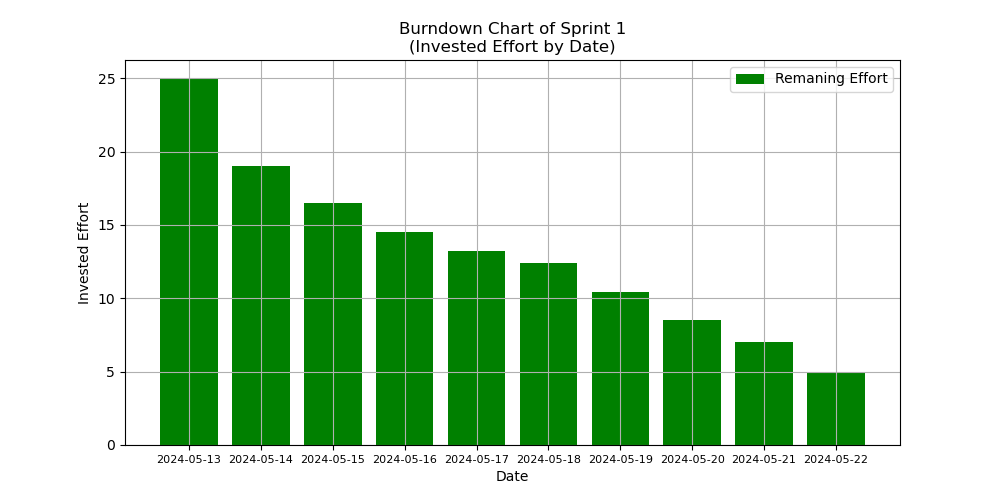
\includegraphics[width=0.9\textwidth]{images/Sprint-1-burndown-chart.png}
\end{figure}


		
	\newpage
	
\end{document}
